\chapter{Exam II}

\begin{problem}[True/False]


%%%%%%%%%%%%%%%%%%%%%%%%%%%%%%%%%%%%
\asktf 

Consider taking the union of two sets with $n$ elements in total
(summed over both sets).  In the worst case, the union operation
performs the most work when the two sets contain an equal number of
elements and less work when one set contains significantly more
elements that the other.

\solt

%%%%%%%%%%%%%%%%%%%%%%%%%%%%%%%%%%%%
\asktf

On an undirected graph if  BFS visits a vertex $v$ at round $r$ (round
start at $0$) then the shortest path from $v$ to the source vertex has
length $r$.

\solt


%%%%%%%%%%%%%%%%%%%%%%%%%%%%%%%%%%%%
\asktf

When BFS visits a vertex $v$, it adds all of its neighbors to the
frontier, which is to be visited in the next round.

\solf

%%%%%%%%%%%%%%%%%%%%%%%%%%%%%%%%%%%%
\asktf

BFS is a natural algorithm for computing topological sort in a directed graph.

\solf



%%%%%%%%%%%%%%%%%%%%%%%%%%%%%%%%%%%%
\asktf
A back-edge is an edge of the DFS-tree that connects a descendant to
an ancestor.
\solf
% a back-edge is a non-tree edge.

%%%%%%%%%%%%%%%%%%%%%%%%%%%%%%%%%%%%
\asktf 

In a DFS of a graph, for any edge $(u,v)$ in the graph, the discovery
time of $u$ is less than the discovery time of $v$.  

\solf


%%%%%%%%%%%%%%%%%%%%%%%%%%%%%%%%%%%%
\asktf 
For any DFS-tree edge $(u,v)$ in a graph, the finish time of $v$ is
less than the finish time of $u$.  
\solt

%%%%%%%%%%%%%%%%%%%%%%%%%%%%%%%%%%%%
\asktf 
Given a graph and the DFS numbers, we can determine the
forward, back, and cross edges by inspecting DFS numbers only.  
\solt

%%%%%%%%%%%%%%%%%%%%%%%%%%%%%%%%%%%%
\asktf

If a graph has negative edge weights, the unmodified Dijkstra's
algorithm for shortest path may loop forever.

\solf

%%%%%%%%%%%%%%%%%%%%%%%%%%%%%%%%%%%%
\asktf

If we run Bellman-Ford on a graph with a negative-weight cycle, then
the algorithm will terminate and indicate that it has found a
negative-weight cycle.

\solf
% It can be unreachable from the source.


%%%%%%%%%%%%%%%%%%%%%%%%%%%%%%%%%%%%
\asktf 

A round of graph contraction with star partitioning (star contraction)
eliminates a constant fraction of vertices and edges.

\solf

% not that of edges.

\end{problem}

%% \input{../../../setstables/graph-representation-adj-tables}
\section{(Sets and Tables) Representing Graphs}
\used{S15 exam2, F16}
%uses new set comprehension syntax




\begin{problem}[Adjacency Tables]

Assume for this problem that we represent a directed graph using an
adjacency table representation, where each vertex is mapped to its set
of neighbors. 

Recall that you can use set comprehension syntax for sets and tables.

\ask[5]
Write out the how the graph would be represented in this
representation using the notation for sets and tables that you have
learned in class.

\begin{center}
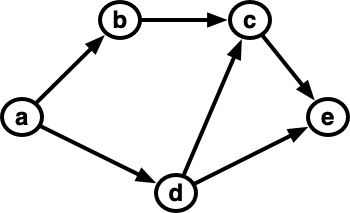
\includegraphics[width=2in]{setstables/digraph-1}
\end{center}

\sol
$\{a \mapsto \{b,d\}, b \mapsto \{c\}, c \mapsto \{e\}, d \mapsto \{c,e\}, e \mapsto \{\} \}$ \\

\notes
\textbf{Common Mistakes}: Forgetting to include $e \mapsto \{\}$. 


\ask[12]
Your goal now is to write a function that given a graph creates
another graph where each pair of edges is shortcut.  That is any edge
in the input graph is also in the output graph, and in addition for
any pair of edges of the form $(u,v),(v,w)$ in the input graph $G$,
there is an additional edge $(u,w)$ in the output.

\begin{lstlisting}[numbers=none]
fun shortcut(G) = 
  let 


    fun f (N,G) = $\underline{~~~~~~~~~~~~~~~~~~~~~~~~~~~~~~~~~~}$



  in   

    $\{u \mapsto f(N,G): (u \mapsto N) \in G\}$

  end

\end{lstlisting}

\sol
Any of the following solutions would work 
\begin{lstlisting}[numbers=none]
fun shortcut(G) = 
  let 
    fun f (N,G) = $N \cup \bigcup_{v \in N} \left(N': v \mapsto N' \in G\right)$
  in   
    $\cset{u \mapsto f(N,G): (u \mapsto N) \in G}$
  end
\end{lstlisting}

\begin{lstlisting}[numbers=none]
fun shortcut(G) = 
  let 
    fun f (N,G) = $N \cup \bigcup_{v \in N} G[v]$
  in   
    $\cset{u \mapsto f(N,G): (u \mapsto N) \in G}$
  end
\end{lstlisting}

\notes
\textbf{Common Mistakes}: Forgetting to include N, the argument passed in into the solution. When writing set notation mixed with SML, forgetting that Table.find returns an option rather than the actual argument. Also, often students forgot to convert between a sequence and a set, which led to using functions such as map on sets.

\end{problem}



%% \newpage
%% \input{../../../dfs/dfs-numbers-1}
\section{(DFS) Numbers}

Given a graph $G = (V,E)$, the traversal order of a depth-first search starting
from $s$ defines a tree $T(G, s)$, known as the \emph{depth-first search tree},
with the following properties:
\begin{enumerate}[itemsep=2pt,topsep=0pt,label=(\roman*),
  labelindent=2\parindent,
  leftmargin=*]
\item $s$ is the root of the tree $T(G,s)$;
\item the tree $T(G,s)$ contains exactly the vertices reachable from $s$; and
\item there is an arc (a directed edge) from $u$ to $v$ if the
  \emph{first} visit to $v$ is
from $u$ (i.e., $u$ calls DFS on $v$ and $v$ hasn't been visited before).
\end{enumerate}

It is easy to record the \emph{discovery time} $d_u$ and
\emph{finishing time} $f_u$ for every vertex.  Starting with a count
of 1, each time a vertex is
first visited (enter) and when a vertex is
last visited (exit) the counter is incremented.  The discovery time
corresponds to the counter when it is first entered, and the finishing
time corresponds to the counter when it last visited.

\begin{problem}
\ask[8]
Run depth-first search on the directed graph below, starting at vertex
A. Whenever there is a choice in the order to explore vertices, use
the vertices in alphabetical order.
For each vertex fill in the corresponding row in the
table with the discovery and finishing
times for that vertex. For example, at the root node $A$, the
counter is $1$ when it is first visited and $12$ when it is finally exited.

\vspace{.1in}
\noindent
\begin{minipage}{.45\textwidth}
\begin{center}
  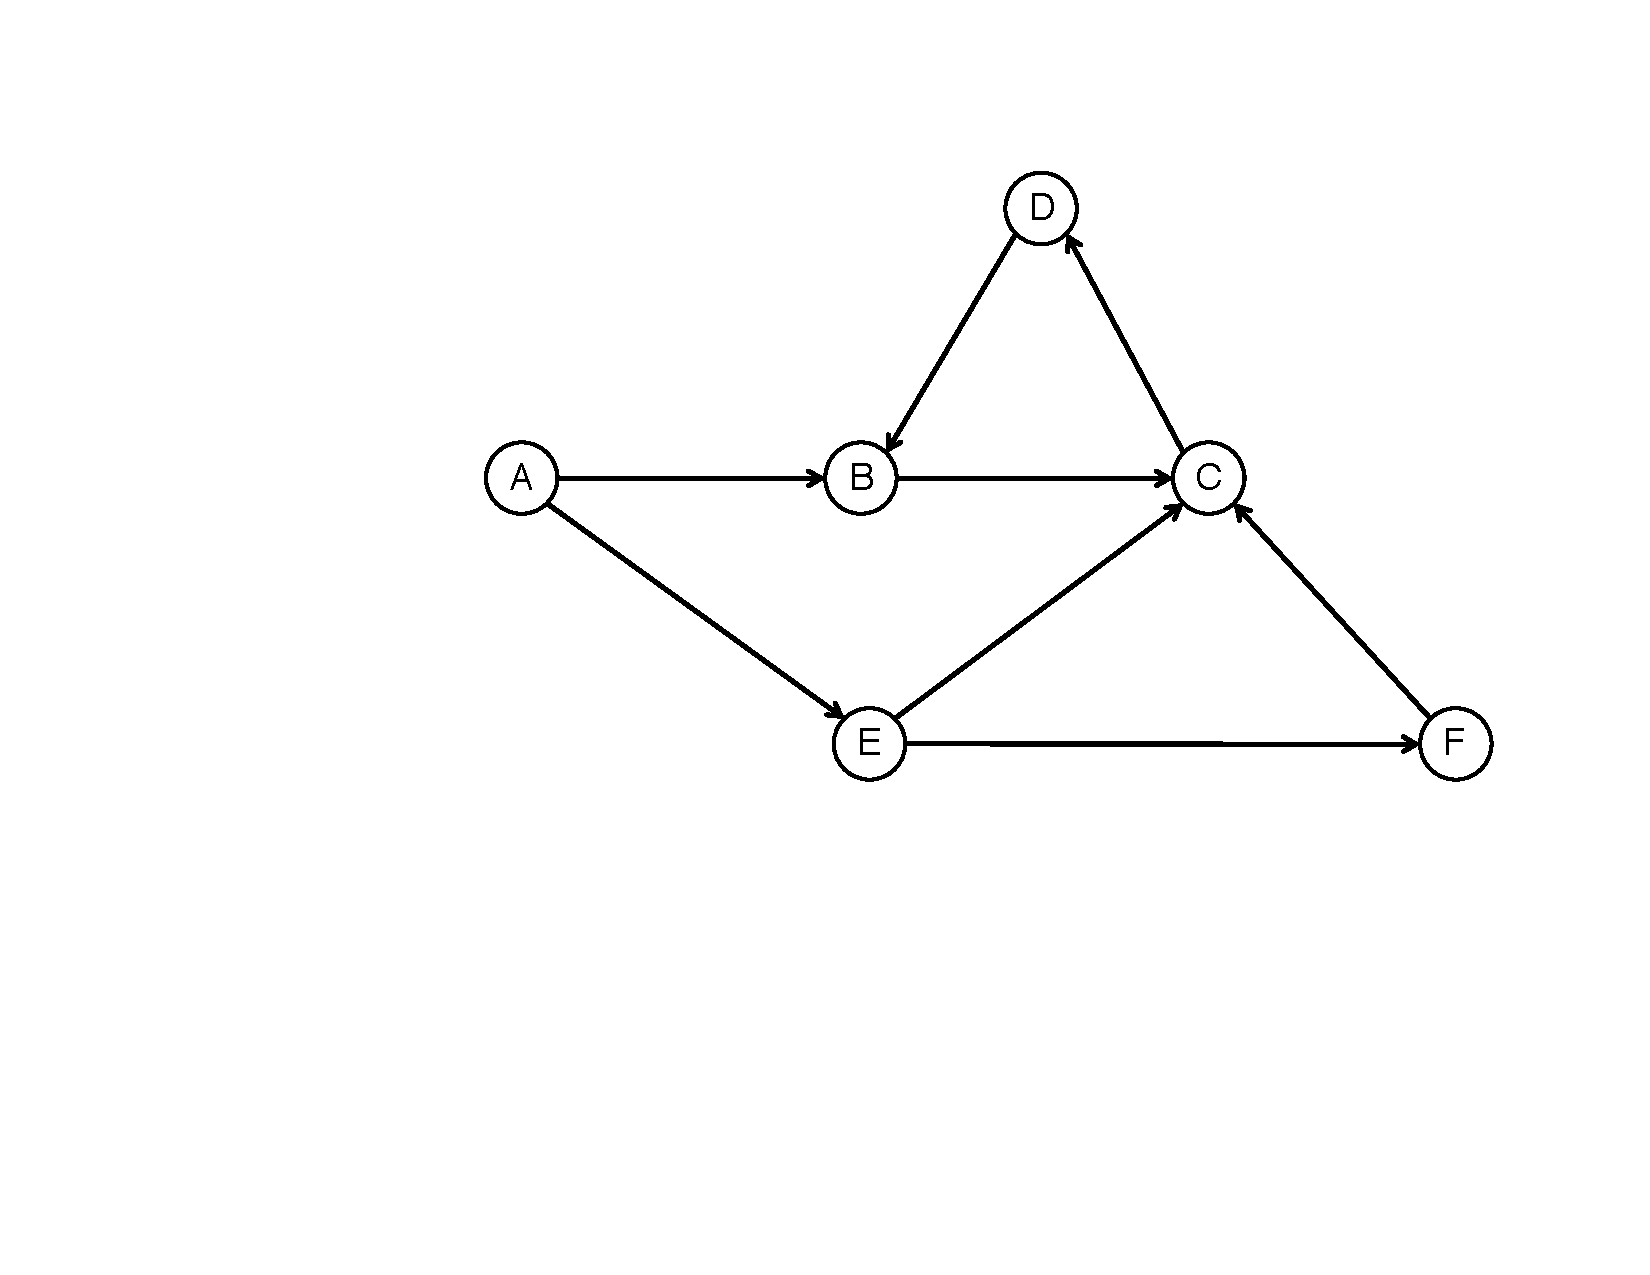
\includegraphics[scale=.45]{dfs/dfs}\\[.2in]
\end{center}
\end{minipage}


\begin{minipage}{.45\textwidth}
  \large
  \begin{center}
    \begin{tabular}{c|c|c}
      Vertex & discovery & finishing\\
      & time & time \\
      \hline \hline
      A & 1 & 12 \\
      \hline
      B & & \\
      \hline
      C & & \\
      \hline
      D & & \\
      \hline
      E & & \\
      \hline
      F & & \\
      \hline
    \end{tabular}
  \end{center}
\end{minipage}

\sol
\begin{minipage}{.45\textwidth}
  \begin{center}
    \begin{tabular}{c|c|c}
       Vertex & discovery & finishing\\
      & time & time \\
      \hline \hline
      A & 1 & 12 \\
      \hline
      B & 2 & 7 \\
      \hline
      C & 3 & 6\\
      \hline
      D & 4 & 5\\
      \hline
      E & 8& 11\\
      \hline
      F & 9& 10\\

    \end{tabular}
  \end{center}
\end{minipage}


\ask[8] On the graph, write next to any edge that is  \textbf{not} a tree edge with
``forward'', ``back'', or ``cross'' depending on whether it is a
forward edge, back edge or cross edge.


\sol
Edges (E, C) and (F, C) are cross edges. Edge (D, B) is a back edge.



\asktf[4] Is it possible to find a topological order of the vertices
for the above graph? Justify your answer.

\solf

\sol
The graph must be a directed acyclic graph in order to
topological sort the vertices.

\end{problem}


%% \input{../../../shortest-paths/shortest-paths-basics}

\section{Shortest Paths, The Basics}
\used{S15 exam2}

This problem concerns several basic properties of shortest paths and
shortest path algorithms that we saw in class, Dijkstra's and
Bellman-Ford.

Throughout assume that the graphs contain no negative edges and are
represented using adjacency sequences,  which map each
vertex to the sequence of out-neighbors and edge weights.

Use $n$ for the number of vertices in the graph and $m$ for the number
of edges.

\begin{problem}[Work and Span]

Let $G$ be a graph and a source vertex $s$ such that all vertices in
the graph are connected via a shortest path to $s$ that contains $k$
or fewer edges.


What is the work and span of an execution of Dijkstra's algorithm on
$G$ and $s$?

\ask  Work:
\sol $O(m\log{n})$

\ask Span:
\sol $O(m\log{n})$



\ask
What is the work and span of an execution of Bellman-Ford algorithm on
$G$ and $s$?

\sol
Work: $O(km)$

\sol
Span : $O(k\log{n})$

\notes
\textbf{Common Mistakes:}
\begin{itemize}
	\item Not recognizing that there are only $k$ rounds of Bellman Ford in this
  scenario.

	\item Including an extra factor of $O(\log n)$ in the work. (This is
  eliminated when the graph is represented by an adjacency sequence.)
\end{itemize}
\end{problem}

\begin{problem}
Recall that a {\em single-pair} shortest path query asks for the
shortest path from a source to a destination.
%

In many applications of shortest paths, we repeat single-pair queries
on the same graph $G = (V,E)$ and often with a small number $k$ of
{\em special} sources, where $k \ll n$ ($k$ is very small relative to
$n$).


One way to take advantage of this use case is to pre-process the graph
in some way to generate some data structure (possibly another graph)
based on the $k$ special sources, and then use this data structure to
answer the shortest path queries.


\ask[4] Describe a preprocessing algorithm that takes a graph
  and the special sources as input and computes the data structure (2-3
  sentences should suffice).  Your preprocessing algorithm should be
  parallel and should perform as little work as possible.


\sol

  Assuming that \textsf{Dijkstra$(G, s)$} returns a mapping of vertices to
  their shortest-path distances (or shortest paths themselves), starting from
  source $s$:
  \[
    \big\langle (\textsf{if $v$ is a special source then Dijkstra$(G,v)$
    else $\bot$}) : v \in V \big\rangle
  \]

%  For each source vertex in the source set, perform Dijkstra, all in
%  parallel.  Create a graph that contains all the vertices of the
%  original graph and a $k(n-1)$ edges from each source to all other
%  vertices, where each edge has a weight that is equal to the shortest
%  path that it represents.
%
%
%  Grading rubric: Using Bellman-Ford is overkill. No more than 1
%  points for that. Instead of the graph, we can also create a table
%  mapping sources do distances (this is the same things as the
%  graph). For efficiency though the table should be represented as a
%  sequence of sequences.  If this is not mentioned, then take out
%  $-1$.

\notes
\textbf{Common Mistakes:}
\begin{itemize}
  \item Not specifying which shortest path algorithm to use.
  \item Using Bellman-Ford rather than Dijkstra. We are guaranteed non-negative
  edge weights, so Bellman-Ford is too expensive.
  \item Ambiguity in describing what happens in parallel.
  \item Unable to guarantee fast query (see below).
\end{itemize}


\ask[4]
State the work and span of your algorithm.


Work: 
\sol $O(n + km\log n)$

Span:
\sol $O(m\ log n)}$


\ask[5]
Describe how to use the data structure resulting from the
preprocessing algorithm to answer quickly and efficiently single-pair
shortest path queries originating at one of the special sources (no
restrictions on the destination)

\notes
\textbf{Common Mistakes:}
\begin{itemize}
	\item Query is too expensive, due to insufficient preprocessing.
	\item Query is unable to distinguish between different source vertices, due
  to simplifications made in the preprocessing step. For example, if all
  sources were combined into a single node, or if they were all connected to
  some new unique source via weight-0 edges.
	\item Attempting to reconstruct paths, resulting in a cost of $O(d)$, where
  $d$ is the diameter of the graph. We should instead just construct paths in
  the preprocessing step.
	\item Incurring a logarithmic lookup cost, due to using tables. Sequences are
  sufficient, and we get constant-time lookup.
\end{itemize}

\sol
If $D$ is the result of the preprocessing step and we are looking for a path
$(s, t)$, then simply perform a lookup: $D[s][t]$.


\ask What is the work of your algorithm
Work: \sol $O(1)$

\ask Span: \sol$O(1)$


\end{problem}


%% \newpage
%% \input{../../../shortest-paths/neighborhoods}

%% \newpage
%% \input{../../../graph-contraction/tree-contraction-2}


%% \end{questions}

%% \newpage
%% \large{\textbf{Scratch Work:}}

%% \vspace*{\fill}


%% \newpage
%% \section*{Appendix: Library Functions}
%% \input{../../../latex/libfuncs}

%% %% this depends on if you want single sided or scratch at the back
%% %%
%%  \newpage
%%  \large{\textbf{Scratch Work:}}

%% %% \vspace*{\fill}

%% \newpage
%% \large{\textbf{Scratch Work:}}

%% \vspace*{\fill}



%% \end{document}
